
\section{Introduction}
\label{sec4:intro}


The shape of life changes on many different time scales.
From generation to generation, populations gradually increase in complexity and relative competency.
At the individual level, organisms grow from a single-celled egg and exhibit extreme postnatal change as they interact with the outside world during their lifetimes.
At a faster time scale still, organisms behave such as to survive and reproduce.

Many organisms manifest different traits as they interact with their environment.
It seems wasteful not to utilize this extra exploration to speed the evolutionary search for good genotypes. 
However, to communicate information from these useful but temporary traits to the genotype requires inverting the generally very complex, nonlinear and stochastic mapping from DNA to phenotype.
Inverting such a function would be exceedingly difficult to compute.
Organisms can, however,
pass on their particular capacity to acquire certain characteristics. 
Thus phenotypic plasticity can affect the direction and rate of evolutionary change by influencing selection pressures.
Although this phenomenon was originally described by Baldwin \cite{baldwin1896new}, Morgan \cite{morgan1896modification} and Waddington \cite{waddington1942canalization}, among others, it has become known as `the Baldwin effect'.
% \cite{simpson1953baldwin}.
In Baldwin's words:
`the most plastic individuals will be preserved to do the advantageous things for which their variations show them to be the most fit, and the next generation will show an emphasis of just this direction in its variations' \cite{baldwin1896new}.
% \begin{quote}
% The most plastic individuals will be preserved to do the advantageous things for which their variations show them to be the most fit, and the next generation will show an emphasis of just this direction in its variations.\cite{baldwin1896new}
% \end{quote}
In a fixed environment, when the `advantageous thing' to do is to stay the same, selection can favor genetic variations which more easily, reliably, or quickly produce these traits. 
This can lead to the genetic determination of a character which in previous generations needed to be developed or learned.


Thirty years ago, Hinton and Nowlan \cite{hinton1987learning} provided a simple computational model of the Baldwin effect that clearly demonstrated how phenotypic plasticity could, under certain conditions, speed evolutionary search without communication to the genotype.
They considered the evolution of a bitstring that is only of value when perfectly matching a predefined target string.
The search space therefore has a single spike of high fitness with no slope leading to the summit.
In such a space, evolution is no better than random search.

Hinton and Nowlan then allowed part of the string to randomly change at an additional (and faster) developmental time scale.
When the genetically specified (nonplastic) portion of the string is correct, there is a chance of discovering the remaining portion in development.	
The speed at which such individuals tend to find the good string will be proportional to the number of genetically determined bits.
When the target string is found, development stops and the individual is rewarded for the amount of remaining developmental time.
This has the effect of creating a gradient of increasing fitness surrounding the correct specification that natural selection can easily climb by incrementally assimilating more correct bits to the genotype.


Hinton and Nowlan imagined the bitstring as specifying the connections of a neural network in a very harsh environment.
We are also interested in this interaction of subsystems unfolding at different time scales, but consider an embodied agent situated in a physically-realistic environment rather than an abstract control system.
This distinction is important as it grounds our hypotheses in the constraints and opportunities afforded by the physical world.
It also allows us to investigate how changes in morphology and control might differentially affect the direction or rate of evolutionary search.
More specifically, it exposes the previously unknown phenomenon of differential canalization reported here.

Inspired by Hinton and Nowlan, Floreano and Mondada \cite{floreano1996plastic} explored the interaction between learning and evolution in mobile robots with a fixed body plan but plastic neural control structure.
They noted that the acquisition of stable behavior in ontogeny did not correspond to stability (no further change) of individual synapses, but rather was regulated by continuously changing synapses which were dynamically stable.
In other words, agents exploited this ontogenetic change for behavior, and this prevented its canalization.
In this paper, we structure development in a way that restricts its exploitation for behavior and thus promotes the canalization of high performing static phenotypes.
Also, the robot's body plan was fixed in Floreano and Mondada's experiments\cite{floreano1996plastic}, whereas in the work reported here, evolution and development may modify body plans.


Several models that specifically address morphological development of embodied agents have been reported in the literature
\cite{dellaert1996developmental,Eggenberger97,Bongard01,miller2004evolving,doursat2009organically}.
However, the relationship between morphological development and evolvability is seldom investigated in such models.
Moreover, there are exceedingly few cases that considered postnatal change to the body plan of an agent (its resting structural form) as it behaves and interacts with the environment through physiological functioning (at a faster time scale).


We are only aware of four cases reported in the literature in which a simulated robot's body was allowed to change while it was behaving.
In the first two cases \cite{ventrella1998designing, komosinski2003framsticks}, it was not clear whether this ontogenetic morphological change facilitated the evolution of behavior.
Later, Bongard \cite{bongard2011morphological} demonstrated how such change could lead to a form of self-scaffolding that smoothed the fitness landscape and thus increased evolvability.
This ontogenetic change also exposed evolution to a wider range of sensor-motor contingencies, which increased robustness to novel environments.
More recently, Kriegman \textit{et al.} \cite{kriegman2017minimal} showed how development can sweep over a series of body plans in a single agent, and subsequent heterochronic mutations canalize the most promising body plan in more morphologically-static descendants.


We are not aware of any cases reported in the literature to date in which a simulated robot's body and control are simultaneously allowed to change while it is behaving.
In this paper, we investigate such change in the morphologies and controllers of soft robots as they are evolved for coordinated action in a simulated 3D environment.
By morphology we mean the current state of a robot's shape, which is slowly changed over the course of its lifetime by a developmental process.
We distinguish this from the controller, which sends propagating waves of actuation throughout the individual, which also affects the instantaneous shape of the robot but to a much smaller degree.
We here refer to these two processes as `morphology' and `control'.
As both processes change the shape, and thus behavior, of the robot, this distinction is somewhat arbitrary.
However, the central claim of this paper, which is that some traits become canalized while others do not, is not reliant on this distinction.


\begin{figure}[t]
\centering
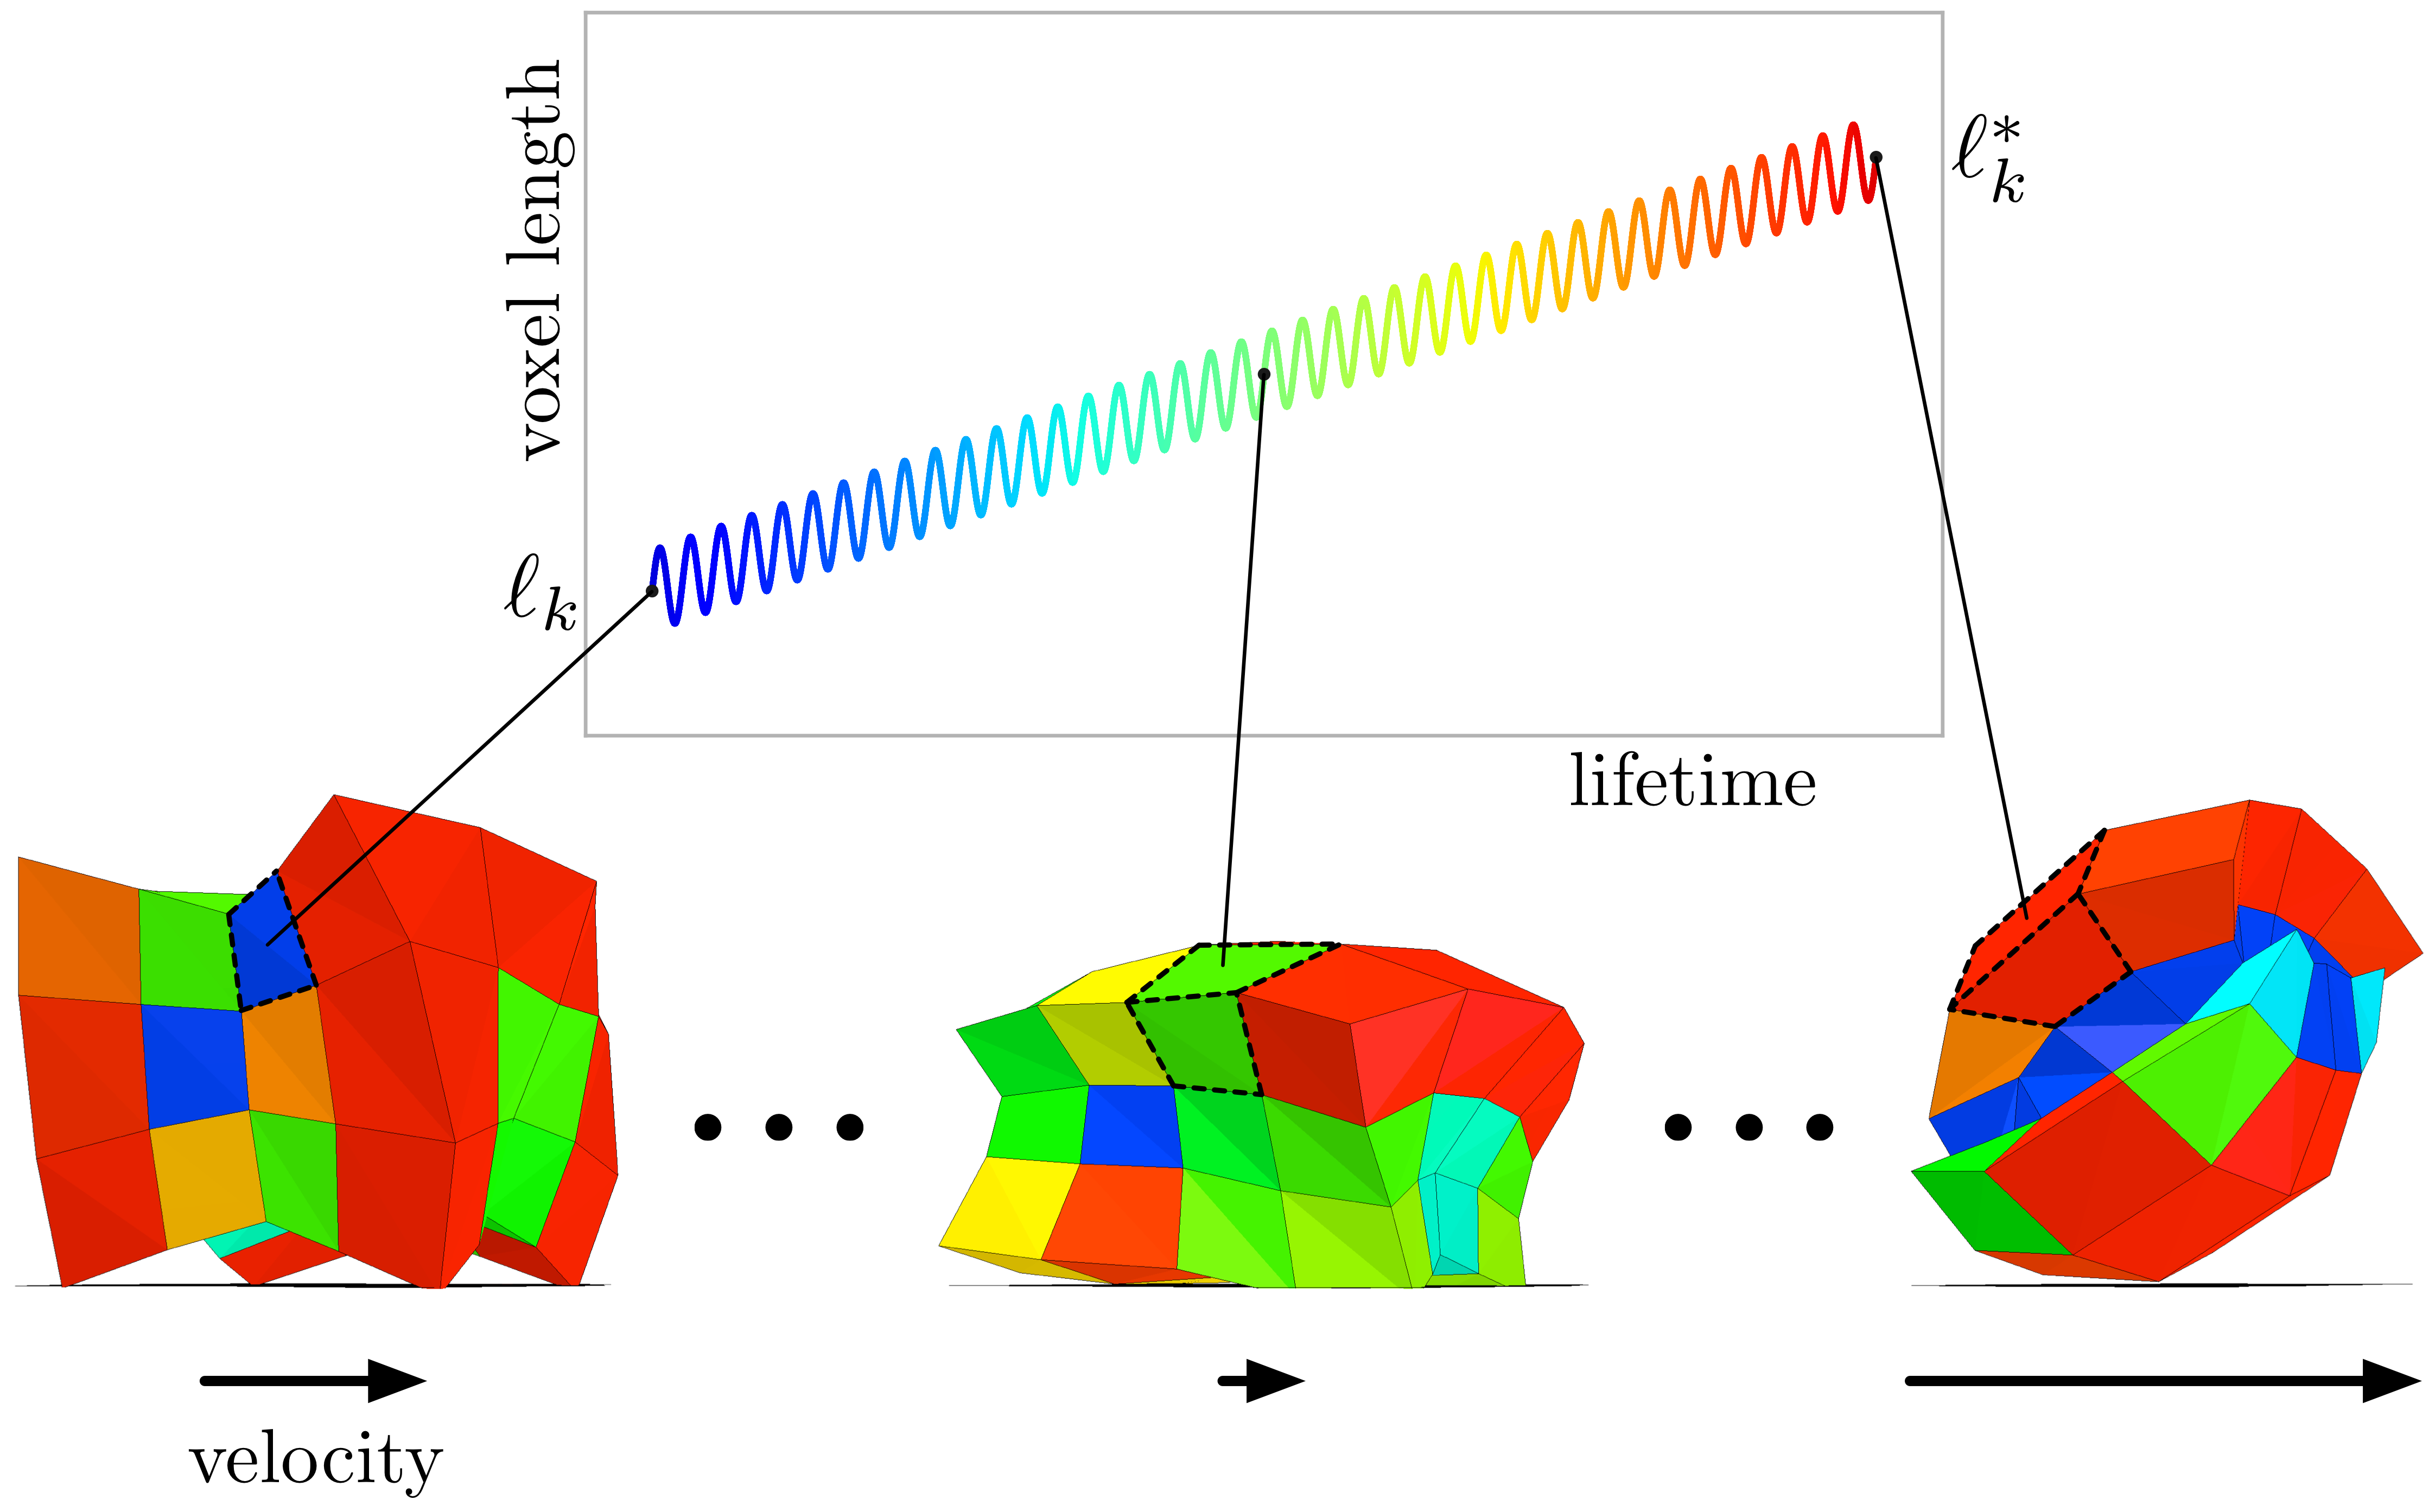
\includegraphics[width=0.8\linewidth]{Chapter04/Fig1}
\caption{\label{fig:blueprint}\textbf{Modeling development.} An evolved soft robot changes its shape during its lifetime (postnatal development), from a walking quadruped into a rolling form. 
Evolution dictates how a robot's morphology develops by setting each voxel's initial ($\ell_k$) and final ($\ell^*_k$) resting length.
The length of a single voxel $k$ is plotted to illustrate its (slower) growth and (faster) actuation processes.
Voxel color indicates the current length of that cell: the smallest voxels are blue, medium sized voxels are green, and the largest voxels are red.
As robots develop and interact with a physically realistic environment, they generate heterogeneous behavior in terms of instantaneous velocity (bottom arrows).
Soft robot evolution, development and physiological functioning can be seen in Supplementary \href{https://youtu.be/Ee2sU-AZWC4}{\color{blue}Video S1}.
}
\end{figure}


We use soft robots because they provide many more degrees of morphological freedom compared to traditional robots composed of rigid links connected by rotary or linear actuators.
This flexibility allows soft robots to accomplish tasks that would be otherwise impossible for their rigid-bodied counterparts, such as squeezing through small apertures \cite{Cheney:2015:ESR:2739480.2754662} or continuously morphing to meet different tasks.
Recent advancements in materials science are enabling the fabrication of 3D-printed muscles \cite{miriyev2017soft} and nervous systems \cite{wehner2016integrated}.
However, there are several challenges to the field of soft robotics, including an overall lack of design intuition:
What should a robot with nearly unbounded morphological possibility look like, and how can it be controlled?
Controllability often depends on precision actuation and feedback authority, but these properties are difficult to maintain in soft materials in which motion in one part of the robot can propagate in unanticipated ways throughout its body \cite{lipson2014challenges}.

We present here a minimally complex but embodied model of morphological and neurological development.
This new model represents an alternative approach to the challenging problem of soft robot design and presents an \textit{in silico} testbed for hypotheses about evolving and developing embodied systems.
This model led to the discovery of differential canalization and how it can increase evolvability.


